\scanpage{66}
d'un corps de base alg. clos, et à prouver donc:

\uline{Lemme}\quad Soit $M$ vectoriel sur $k$
\deleted{\unsure{parf.}}\inserted{alg.} clos de car $p$,
muni de $F_M:M^{(p)}\xrightarrow{\sim}M$.
Soit $E=\{x\in M,\ Fx^{(p)}=x\}$. Alors
$E\otimes_{\mathbb F_p}k\xrightarrow{\sim}M$.
\figure{\begin{tikzpicture}\draw (0,0)--(0,-.7);\end{tikzpicture}}

\figure{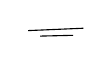
\begin{tikzpicture}
\draw (0,0)--(.7,.03); \draw (.15,-.07)--(.57,-.06);
\end{tikzpicture}}

$\mathcal C$ catégorie des schémas en \inserted{$p$-}groupes
\deleted{\unsure{finis et étales}} \inserted{finis étales} sur $S$
\inserted{i.e. des faisceaux en $p$-groupes loc. constants de t.f.}
\deleted{\unsure{catégorie des schémas}}

$\mathcal C'$ catégorie des \deleted{schémas}
\inserted{faisceaux} en $W_S^{\unsure{\mathrm{can}}}$-modules $M$
loc. isom à une somme de copies de $W_{nS}$, munis
$\deleted{\unsure{de}}\ M^{(p)}\xrightarrow[\sim]{F_M}M$.
\margin{Zar ou fppf, c'est \unsure{kif kif}}
\figure{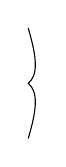
\begin{tikzpicture}
\draw (0,.7)..controls(.12,.3)and(.12,.1)..(0,0)
..controls(.12,-.1)and(.12,-.3)..(0,-.7);
\end{tikzpicture}}

$\mathcal C''$ catégorie des schémas en $W_S$-modules lisses

\diagram{\begin{tikzcd}[ampersand replacement=\&]
\mathcal C\arrow[r,"\varphi"]\arrow[dr,"\psi"']\&
\mathcal C'\arrow[d,"i\ \unsure{\sim}"]\\
\&\mathcal C''
\end{tikzcd}}

$\varphi(E)=E\otimes_{\mathbb Z_p}W_S^{\unsure{\mathrm{can}}}$
avec le $F$ qu'on devine

$i(M)=$ \deleted{faisceau en groupes}
\inserted{schéma} représentant le faisceau\dots

$\psi(E)=E\otimes_{\mathbb Z_p}W_S$
\margin{76}
